\documentclass[12pt,a4paper]{article}
\usepackage[utf8]{inputenc} % inutile avec XeLaTeX/LuaLaTeX
\usepackage[T1]{fontenc}
\usepackage{amsmath,amssymb,mathrsfs,tikz,times,pifont}
\usepackage{enumitem}
\usepackage{multicol}
\usepackage{lmodern}
\newcommand\circitem[1]{%
\tikz[baseline=(char.base)]{
\node[circle,draw=gray, fill=red!55,
minimum size=1.2em,inner sep=0] (char) {#1};}}
\newcommand\boxitem[1]{%
\tikz[baseline=(char.base)]{
\node[fill=cyan,
minimum size=1.2em,inner sep=0] (char) {#1};}}
\setlist[enumerate,1]{label=\protect\circitem{\arabic*}}
\setlist[enumerate,2]{label=\protect\boxitem{\alph*}}
\everymath{\displaystyle}
\usepackage[left=1cm,right=1cm,top=1cm,bottom=1.7cm]{geometry}
\usepackage[colorlinks=true, linkcolor=blue, urlcolor=blue, citecolor=blue]{hyperref}
\usepackage{array,multirow}
\usepackage[most]{tcolorbox}
\usepackage{varwidth}
\usepackage{float}
\tcbuselibrary{skins,hooks}
\usetikzlibrary{patterns}

\usepackage{pgfplots}
\pgfplotsset{compat=1.15}
\usepackage{mathrsfs}

\usepackage{amsmath}
\usepackage{amsfonts}
\usepackage{amssymb}
\usepackage{tkz-tab}
\usepackage{mdframed}
\usepackage{tikz}
\usetikzlibrary{arrows, shapes.geometric, fit}

% Commande pour la couleur d'accentuation
\newcommand{\myul}[2][black]{\setulcolor{#1}\ul{#2}\setulcolor{black}}
\newcommand\tab[1][1cm]{\hspace*{#1}}

%\usepackage[margin=2cm]{geometry}
\usepackage{eso-pic}         % Pour ajouter des éléments en arrière-plan

\usepackage{enumitem}
%---------------------------------------
% Définir un compteur pour les exemples
\newcounter{exemple}

% Définir la commande \exemple pour afficher un exemple numéroté
\newcommand{\exemple}{%
  \refstepcounter{exemple}% Incrémenter le compteur
  \textbf{\textcolor{orange}{Exemple \theexemple : }} \ignorespaces
}
%---------------------------------------
\newcounter{solution}

% Définir la commande \solutione pour afficher un solution numéroté
\newcommand{\solution}{%
  \refstepcounter{solution}% Incrémenter le compteur
  \textbf{\textcolor{orange}{Solution \thesolution : }} \ignorespaces
}
%---------------------------------------
\definecolor{myorange}{rgb}{1.0, 0.8, 0.0}

% Définir un compteur pour les exercices d'application
\newcounter{exerciceapp}

% Définir la commande pour afficher un exercice d'application numéroté
\newcommand{\exerciceapp}{%
  \refstepcounter{exerciceapp}%
  \textbf{\textcolor{myorange}{Exercice d'application \theexerciceapp :}} \ignorespaces
}
%--------------------------------------
% Définir un compteur pour les exercices d'application
\newcounter{correction}

% Définir la commande pour afficher un correction exercice d'application numéroté
\newcommand{\correction}{%
  \refstepcounter{correction}%
  \textbf{\textcolor{myorange}{Correction \thecorrection :}} \ignorespaces
}
%--------------------------------------
% Définir un compteur pour les remarque d'application
\newcounter{remarque}

%----------------------------------------
\definecolor{myorange1}{rgb}{1.0, 1.5, 0}
% Définir la commande pour afficher un remarque numéroté
\newcommand{\remarque}{%
  \refstepcounter{remarque}%
  \textbf{\textcolor{myorange1}{Remarque \theremarque :}} \ignorespaces
}

% Commande pour ajouter du texte en arrière-plan
\AddToShipoutPicture{
    \AtTextCenter{%
        \makebox[0pt]{\rotatebox{45}{\textcolor[gray]{0.6}{\fontsize{5cm}{5cm}\selectfont PGB}}}
    }
}

\begin{document}
% En-tête personnalisée
\begin{center}
    \Large\textbf{\underline{\textcolor{red}{Dénombrement}}}\\[-0.1cm]
    \normalsize\textbf{Prof : M. BA} \hfill \textbf{Classe : TS2}\\[-0.1cm]
    \textbf{Année scolaire : 2025 -- 2026}
\end{center}

\begin{enumerate}[label=\Roman*., font=\bfseries\color{red}]
    \item \textbf{Rappel sur la théorie des ensembles}
    \begin{enumerate}
        \item Définition et vocabulaire (Éléments, ensembles finis, cardinal, ensemble vide)
        Un ensemble est un regroupement d'objets défini par une caractéristique commune ou par une énumération complète.

Chaque objet de l'ensemble est appelé un \textcolor{red}{élément}.

Un ensemble est dit \textcolor{red}{fini} s'il est constitué d'un nombre fini d'éléments et ce nombre est appelé le \textcolor{red}{cardinal} de l'ensemble.

Il existe un ensemble qui ne contient aucun élément, il est appelé \textcolor{red}{l'ensemble vide} noté $\varnothing$.

\textbf{\underline{\exemple}}

\[
E=\{a,b,c,d,e\}, \qquad 
J=\{x\in\mathbb{R}\mid x\geq 2\}
\]

\[
K=\{1,2,3,4,5,6\}, \qquad 
P=\{n\in\mathbb{N}\mid 10\leq n\leq100\}
\]

\[
E,\;K \text{ et } P \text{ sont des ensembles finis}
\]

\[
\mathrm{card}(E)=5 \;;\quad 
\mathrm{card}(P)=91 \;;\quad 
\mathrm{card}(K)=6 \;;\quad 
\mathrm{card}(\varnothing)=0
\]
        \item Partie d'un ensemble (Sous-ensembles et ensemble des parties $\mathcal{P}(E)$)

Soit $E$ un ensemble fini de cardinal $n$.

$A$ est dit un sous-ensemble ou une partie de $E$ ssi $x \in A \implies x \in E \iff A \subset E$ ($A$ incluse dans $E$). 

On écrit que $A \in \mathcal{P}(E)$ où $\mathcal{P}(E)$ est l'ensemble des sous-ensembles de $E$ et :
\[ \text{card } \mathcal{P}(E) = 2^{\text{card } E} \implies \text{card } \mathcal{P}(E) = 2^n \]

\textbf{\underline{\exemple}}

Soit $E = \{1; 2; 3\}$ \\
$\text{card } E = 3$ \\
$\text{card } \mathcal{P}(E) = 2^3 = 8$

\[ \mathcal{P}(E) = \{E, \emptyset, \{1\}, \{2\}, \{3\}, \{1; 2\}, \{1; 3\}, \{2; 3\}\} \]
        \item Complémentaire d'un ensemble

Soit $E$ un ensemble fini non vide, $A$ un sous-ensemble de $E$.

On appelle complémentaire de $A$, l'ensemble des éléments de $E$ qui ne sont pas dans $A$ noté $\overline{A}$.
\[ x \in \overline{A} \iff x \in E \text{ et } x \notin A \]

\begin{center}
    \fbox{$\text{card } \overline{A} = \text{card } E - \text{card } A$}
\end{center}       
       
        \item Réunion et Intersection (Définitions, propriétés et diagrammes de Venn)
        Soit $A$ et $B$ deux sous-ensembles de $E$.

La réunion de $A$ et $B$ est un sous-ensemble de $E$ noté : 
$A \cup B = \{x \in E / x \in A \text{ ou } x \in B\}$
\[ x \in A \cup B \iff x \in A \text{ ou } x \in B \]

\subsection*{Propriétés :}
\begin{itemize}
    \item $A \cup B \subset E$ \hfill $\circ$ $A \cup E = E$
    \item $A \subset A \cup B$ \hfill $\circ$ $A \cup \overline{A} = E$
    \item $B \subset A \cup B$ \hfill $\circ$ $A \cup \emptyset = A$
\end{itemize}

L'intersection de $A$ et $B$ est un sous-ensemble de $E$ noté :
$A \cap B = \{x \in E / x \in A \text{ et } x \in B\}$
\[ x \in A \cap B \iff x \in A \text{ et } x \in B \]
\subsection*{Propriétés :}
\begin{itemize}
    \item $A \cap B \subset E$ \hfill $\circ$ $A \cap B \subset A$
    \item $A \cap E = A$ \hfill $\circ$ $A \cap B \subset B$
    \item $A \cap \overline{A} = \emptyset$ \hfill $\circ$ $A \cap \emptyset = \emptyset$
\end{itemize}


% Code pour le diagramme :
\begin{center}
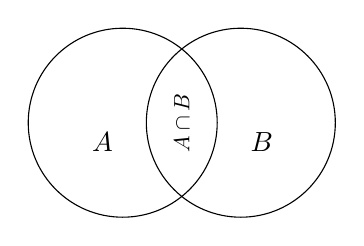
\begin{tikzpicture}[fill opacity=0.3]
    % Cercle A
    \draw (0,0) circle (1.2cm) node[below left, opacity=1] {$A$};
    % Cercle B
    \draw (1.5,0) circle (1.2cm) node[below right, opacity=1] {$B$};
    % Zone d'intersection (A inter B)
    \node at (0.75,0) [opacity=1, scale=0.8, rotate=90] {$A \cap B$};
\end{tikzpicture}
\end{center}

\[ \text{card}(A \cup B) = \text{card } A + \text{card } B - \text{card}(A \cap B) \]

% Note : Pour le diagramme de Venn, on utilise généralement l'environnement tikz, 
% mais voici la transcription textuelle de la suite :

        \item Différence de deux ensembles (Différence simple et différence symétrique $\Delta$)

Soit $A$ et $B$ deux sous-ensembles de $E$.

On appelle la différence entre $A$ et $B$ le sous-ensemble de $E$ noté :

$A \setminus B$ (on lit $A$ sans $B$) : 
$x \in A \setminus B \implies x \in A \text{ et } x \notin B$

$A \setminus B = A \cap \overline{B}$

\[ \text{card}(A \setminus B) = \text{card } A - \text{card}(A \cap B) \]

On appelle différence symétrique le sous-ensemble de $E$ noté :
\[ A \Delta B = (A \setminus B) \cup (B \setminus A) \]
\[ A \Delta B = (A \cup B) \setminus (A \cap B) \]

\begin{center}
    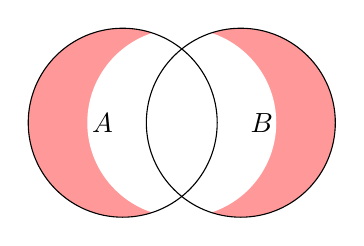
\begin{tikzpicture}[fill opacity=0.4]
        % Zones colorées (différence symétrique)
        \fill[red] (0,0) circle (1.2cm);
        \fill[red] (1.5,0) circle (1.2cm);
        \fill[white, opacity=1] (0.75,0) circle (1.2cm); % On "efface" l'intersection
        \begin{scope}
            \clip (0,0) circle (1.2cm);
            \fill[white, opacity=1] (1.5,0) circle (1.2cm);
        \end{scope}
        
        % Contours
        \draw (0,0) circle (1.2cm) node[left, opacity=1] {$A$};
        \draw (1.5,0) circle (1.2cm) node[right, opacity=1] {$B$};
    \end{tikzpicture}
\end{center}

\begin{center}
    \fbox{$\text{card}(A \Delta B) = \text{card } A + \text{card } B - 2 \text{ card}(B \cap A)$}
\end{center}
\textbf{\underline{\exemple}}

Dans une classe de 45 élèves, 33 ont la moyenne en PC et 24 ont la moyenne en math, 20 élèves ont la moyenne en math et en PC.

\begin{enumerate}
    \item Calculer le nombre d'élèves qui ont la moyenne en Math ou PC.
    \item Calculer le nombre d'élèves qui ont la moyenne qu'en une seule des deux matières.
    \item Calculer le nombre d'élèves qui n'ont la moyenne ni en Math ni en PC.
\end{enumerate}

On notera par $A$ l'ensemble des élèves qui ont la moyenne en PC, $B$ ceux en maths.

\textbf{\underline{\solution}}

\textbf{Données :}
Soit $E$ l'ensemble des élèves de la classe.
\begin{itemize}
    \item $card(E) = 45$ (Effectif total)
    \item $card(A) = 33$ (Moyenne en PC)
    \item $card(B) = 24$ (Moyenne en Math)
    \item $card(A \cap B) = 20$ (Moyenne en Math et en PC)
\end{itemize}

\begin{enumerate}
    \item \textbf{Nombre d'élèves qui ont la moyenne en Math ou PC :}
    On cherche le cardinal de l'union $card(A \cup B)$.
    \[ card(A \cup B) = card(A) + card(B) - card(A \cap B) \]
    \[ card(A \cup B) = 33 + 24 - 20 = 37 \]
    Il y a \textbf{37 élèves} qui ont la moyenne dans au moins une des deux matières.

    \item \textbf{Nombre d'élèves qui ont la moyenne qu'en une seule des deux matières :}
    
    \textbf{Nombre d'élèves qui ont la moyenne qu'en Math :}
    
    Il s'agit de l'ensemble $B$ privé de l'intersection.
    \[ card(B \text{ uniquement}) = card(B) - card(A \cap B) \]
    \[ card(B \text{ uniquement}) = 24 - 20 = 4 \]
    Il y a \textbf{4 élèves} qui ont la moyenne uniquement en Math.

    \textbf{Nombre d'élèves qui ont la moyenne qu'en PC :}
    
     Il s'agit de l'ensemble $A$ privé de l'intersection.
    \[ card(A \text{ uniquement}) = card(A) - card(A \cap B) \]
    \[ card(A \text{ uniquement}) = 33 - 20 = 13 \]
    Il y a \textbf{13 élèves} qui ont la moyenne uniquement en PC.
    
    On additionne ceux qui n'ont que la PC et ceux qui n'ont que les Math.
    \begin{itemize}
        \item Uniquement PC : $13$
        \item Uniquement Math : $4$
    \end{itemize}
    Total : $13 + 4 = 17$.
    Il y a \textbf{17 élèves} qui ont la moyenne dans une seule matière.

    \item \textbf{Nombre d'élèves qui n'ont la moyenne ni en Math ni en PC :}
    On cherche le complémentaire de l'union dans l'ensemble total $E$.
    \[ card(\overline{A \cup B}) = card(E) - card(A \cup B) \]
    \[ card(\overline{A \cup B}) = 45 - 37 = 8 \]
    Il y a \textbf{8 élèves} qui n'ont aucune des deux moyennes.
\end{enumerate}

\item Produit Cartésien (Propriétés des cardinaux de $A \times B$ et $A^n$)

\textbf{Propriétés :}

\( \text{card}(A \times B) = \text{card } A \times \text{card } B \)

\( \text{card}(A^n) = (\text{card } A)^n, \quad \forall n \in \mathbb{N}, n \ge 2 \)

\textbf{\underline{\exemple}}

Une entreprise fabrique des valises avec des codes de sécurité constitués de 2 lettres suivies de 2 chiffres.

\begin{enumerate}
    \item Calculer le nombre de codes possibles pour un client.
    \item Calculer le nombre de codes commençant par une voyelle et finissant par un chiffre impair.
\end{enumerate}

\textbf{\underline{\solution}}  
      
\item \textbf{Les outils du dénombrement} 
\begin{enumerate}
\item La $p$-liste

        \begin{itemize}
            \item \textbf{Définition et caractéristiques (Ordre et répétition)}
            
            Soit $E$ un ensemble fini non vide de cardinal $n$, $p$ un nombre entier naturel.

On appelle $p$-liste d'éléments de $E$ toute liste de longueur $p$ constituée des éléments de $E$ distincts ou identiques.

Une $p$-liste de $E$ est un élément de $E^p$.	

\textbf{\underline{\exemple}}

Soit $E = \{1, 2, 3, a, b\}$

$(1; 2), (2; 2), (3; a), (a; a) \dots$ etc sont des 2-listes de $E$.

$(1; 1; 2), (1; 3; a), (a; a; a), (b; 1; 3) \dots$ etc sont des 3-listes de $E$.

$(1; 1; a; 1; 3; 2; a)$ est une 7-liste de $E$.

        \textbf{Remarque :} 
        
        Une $p$-liste est caractérisée par l'importance de la position et la possibilité de répétition d'élément.

            \item \textbf{Propriété du dénombrement ($n^p$)}
            
            Soit $E$ un ensemble fini de card $n$, $p$ un nombre entier naturel non nul, le nombre de $p$-listes de $E$ est égal à $n^p$.	
        \end{itemize}
         \item Le $p$-arrangement
        \begin{itemize}
            \item \textbf{Définition et caractéristiques (Ordre sans répétition)]}
            
            Soit $E$ un ensemble fini non-nul de card $n$ ; $p$ un entier naturel non nul tel que $1 \le p \le n$. 

On appelle $p$-arrangement de $E$ toute liste de longueur $p$ constituée des éléments distincts de $E$.

Un $p$-arrangement est une $p$-liste sans répétition d'élément.

\textbf{\underline{\exemple}}

Soit $E = \{1; 2; 3; 4; 5\}$

$12 ; 14 ; 41 ; 52 ; 32 ; 15 \dots$ etc sont des $2$-arrangements de $E$

$145 ; 134 ; 152 ; 543 \dots$ ets sont des $3$-arrangements de $E$

\textbf{Remarque :} 

Un arrangement est caractérisé par l'importance de la position (\textit{l'ordre}) et l'absence de répétition.

\textbf{\underline{Propriété :}}

Soit $E$ un ensemble fini non vide de cardinal $n$, $p$ un entier naturel tel que $1 \le p \le n$. Le nombre de $p$-arrangement de $E$ est noté : 
\begin{center}
    \fbox{$A_n^p = n(n-1)\dots(n-p+1)$}
\end{center}

\textbf{\underline{Notation avec factorielles :}}

Le nombre de $p$-arrangements de $n$ éléments peut aussi s'écrire à l'aide des factorielles :
\begin{center}
    \fbox{$A_n^p = \frac{n!}{(n-p)!}$}
\end{center}

\textbf{Cas particulier : Permutations}
Si $p = n$, on parle de permutation de $n$ éléments.
\[ A_n^n = n! \]

\textbf{\underline{\exemple}}

$A_7^2 = 7 \times 6 = 42$

$A_{10}^8 = 10 \times 9 \times 8 \times 7 \times 6 \times 5 \times 4 \times 3 = 1\,814\,400$

$A_8^3 = 8 \times 7 \times 6 = 336$
\textbf{Définition de la factorielle}

Soit $n \in \mathbb{N}, n \ge 2$, on appelle \textbf{factorielle de $n$} le nombre noté $n!$ défini par :
\[ n! = n(n-1)\dots \times 1 \]

\begin{center}
    \fbox{$1! = 1$} \quad \fbox{$0! = 1$}
\end{center}

\textbf{\underline{\exemple}}

$5! = 5 \times 4 \times 3 \times 2 \times 1$

$4! = 4 \times 3 \times 2 \times 1$

$7! = 7 \times 6 \times 5 \times 4 \times 3 \times 2 \times 1$

\color{red}{Propriétés :}

$\forall n \in \mathbb{N} ; n \ge 2 $

$n! = n(n - 1)!$

{\color{red}\fboxsep=10pt
\fbox{\Large $A_n^p = \frac{n!}{(n-p)!}$}}


$A_n^0 = 1$

$A_n^1 = n$

$A_n^n = n!$

$A_n^{n-1} = n!$
            \item \textbf{Formule de calcul ($A_n^p$) et notation avec factorielles}
        \end{itemize}
\item La Permutation

Soit $E$ un ensemble fini de cardinal $n$ non vide, on appelle permutation de $E$ toute liste de longueur $n$ constituée des $n$ éléments de $E$. Donc une permutation est un $n$-arrangement de $E$.
\begin{itemize}
            \item Exemple
            
            Soit $E = \{1; 2; 3\}$
$123; 213; 312; 231; 132$ sont des permutations de $E$
            \item Propriété
            
            Le nombre de permutation de $E$ est égale à \underline{{\color{red}$n!$}}
            \item Application : Les Anagrammes (Cas des lettres distinctes et répétées)
            
            Deux mots sont dits des anagrammes s'ils s'écrivent avec les mêmes lettres mais disposées différemment.
            
            \exemple
            
{\color{red}ASTOU} et SATOU \\
CHIEN et {\color{red}NICHE}

\begin{itemize}
    \item Si un mot est constitué de $n$ lettres distinctes, le nombre d'anagrammes possibles avec les lettres du mot est égale à {\color{red}$n!$}
    \item Si un mot est constitué de $n$ lettres dont quelques unes se répètent le nombre d'anagramme possible avec les lettres du mot est égale à {\color{red}$n!$} divisé par le produit des factorielles du nombre de fois que chaque lettre se répète.
\end{itemize}
            \item Exemple
            
- Donner le nombre d'anagramme possible avec les lettres du mot "{\color{red}ASTOU}"

- Donner le nombre d'anagramme possible avec les lettres du mot "SCIENCES"

\vspace{0.5cm}

\begin{itemize}
    \item $N = {\color{red}5!} = 120$
    \item $M = \frac{8!}{{\color{red}2!2!2!}} = \frac{8!}{8} = 5040$
\end{itemize}

\end{itemize}
 
\item La Combinaison
        \begin{itemize}
            \item Définition et caractéristiques (Sans ordre ni répétition)
Soit $E$ un ensemble fini non vide de cardinal $n$, $P \in \mathbb{N} / P \le n$. On appelle {\color{red}combinaison} de $p$ éléments de $E$ tout sous ensemble de $E$ de cardinal $P$.

            \item Formule de calcul ($C_n^p$)
            
            \exemple
            
            Soit $E = \{1, 2, 3, 4\}$
            
$\{1; 2\}, \{2; 3\}, \{4; 3\}, \{2; 4\}$ sont des \textbf{2-sous-combinaison} de $E$

$\{1; 2; 3\}, \{2; 3; 4\}, \{1; 2; 4\}, \{1; 3; 4\}$ sont \textbf{3-combinaison} de $E$

$\{1; 2; 3; 4\}$ est la \textbf{seule 4-combinaison} de $E$

            \item Remarque (Symétrie, valeurs particulières)
            
            Une combinaison est caractérisée par le fait que la position n'est pas importante et l'absence de répétition d'éléments.
            
            \item Propriétés
            
            Soit $E$ un ensemble fini non vide de cardinal $n$, $P \in \mathbb{N} / P \le n$

Le nombre de $P$-combinaisons de $E$ est noté $C_n^P$ défini : 
\begin{center}
    \fbox{$C_n^P = \frac{n!}{P!(n-P)!} = \frac{A_n^P}{P!}$}
\end{center}
            \item Relation de Pascal ($C_{n-1}^{p-1} + C_{n-1}^p = C_n^p$)
            
            \exemple
            
            $C_7^3 = \frac{7!}{3!(7-3)!} = \frac{7 \times 6 \times 5}{3 \times 2} = 35$

\vspace{0.5cm}

$C_{10}^2 = \frac{10!}{2!(10-2)!} = \frac{10 \times 9}{2} = 45$

\vspace{0.5cm}

$C_{11}^7 = \frac{11!}{7!(11-7)!} = \frac{11!}{7! \, {\color{red}4!}} = \frac{11 \times 10 \times 9 \times 8}{4 \times 3 \times 2} = 330$

$C_n^0 = 1$

$C_n^1 = n$

$C_n^n = 1$

$C_n^{n-p} = C_n^p$

\begin{center}
    {\color{red}
    \fboxsep=10pt
    \fbox{$C_{n-1}^{p-1} + C_{n-1}^p = C_n^p$}
    }
\end{center}

En effet
$C_n^0 = \frac{n!}{0!(n-0)!} = \frac{n!}{n!} = 1$

\vspace{0.4cm}

$C_n^1 = \frac{n!}{1!(n-1)!} = \frac{n \times (n-1)!}{(n-1)!} = n$

\vspace{0.4cm}

$C_n^n = \frac{n!}{n!(n-n)!} = \frac{n!}{n! 0!} = \frac{n!}{n!} = 1$

\vspace{0.4cm}

$C_n^{n-p} = \frac{n!}{(n-p)!(n-n+p)!} = \frac{n!}{(n-p)! p!} = C_n^p$

\vspace{0.4cm}

$C_{n-1}^{p-1} + C_{n-1}^p = \frac{(n-1)!}{(p-1)!(n-1-p+1)!} + \frac{(n-1)!}{p!(n-1-p)!}$

\vspace{0.2cm}

$\quad \quad \quad \quad \quad = \frac{(n-1)!}{(p-1)!(n-p)!} + \frac{(n-1)!}{p!(n-p-1)!}$

\vspace{0.4cm}

or $(n-p)! = (n-p)(n-p-1)!$
$p! = p(p-1)!$

\[
\begin{aligned}
C_{n-1}^{p-1} + C_{n-1}^p &= \frac{(n-1)!}{\frac{p!}{p}(n-p)!} + \frac{(n-1)!}{p!\frac{(n-p)!}{(n-p)}} \\
&= \frac{p(n-1)!}{p!(n-p)!} + \frac{(n-p)(n-1)!}{p!(n-p)!} \\
&= \frac{p(n-1)! + (n-p)(n-1)!}{p!(n-p)!} \\
&= \frac{(n-1)![p + (n-p)]}{p!(n-p)!} = \frac{(n-1)!n}{p!(n-p)!} \\
&= \frac{n!}{p!(n-p)!} = C_n^p
\end{aligned}
\]
\end{itemize}  
\item Triangle de Pascal

\begin{center}
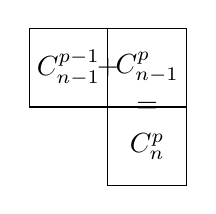
\begin{tikzpicture}
    % Grille pour le schéma de Pascal
    \draw (0,1) rectangle (1,2) node[pos=.5] {$C_{n-1}^{p-1}$};
    \draw (1,1) rectangle (2,2) node[pos=.5] {$C_{n-1}^p$};
    \draw (1,0) rectangle (2,1) node[pos=.5] {$C_n^p$};
    
    % Signe + et =
    \node at (1,1.5) {$+$};
    \node at (1.5,1) {$=$};
\end{tikzpicture}
\end{center}

\begin{center}
\begin{tabular}{|c|c|c|c|c|c|c|c|}
\hline
$n \backslash p$ & 0 & 1 & 2 & 3 & 4 & 5 & 6 \\ \hline
0 & 1 & & & & & & \\ \hline
1 & 1 & 1 & & & & & \\ \hline
2 & 1 & 2 & 1 & & & & \\ \hline
3 & 1 & 3 & 3 & 1 & & & \\ \hline
4 & 1 & 4 & 6 & 4 & 1 & & \\ \hline
5 & 1 & 5 & 10 & 10 & 5 & 1 & \\ \hline
6 & 1 & 6 & 15 & 20 & 15 & 6 & 1 \\ \hline
\end{tabular}
\end{center}
\item Binome De NEWTON

     Soient $a$ et $b$ deux réels, $n \in \mathbb{N}, n \ge 1$

\begin{center}
    {\color{red}
    \fboxsep=10pt
    \fbox{$\displaystyle (a+b)^n = \sum_{k=0}^{n} C_n^k a^{n-k}b^k$}
    }
\end{center}

$(a+b)^n = {\color{red}C_n^0} a^n + {\color{red}C_n^1} a^{n-1}b + {\color{red}C_n^2} a^{n-2}b^2 + \dots + {\color{red}C_n^{n-1}} ab^{n-1} + {\color{red}C_n^n} b^n$

\exemple

$(a+b)^2 = a^2 + 2ab + b^2$ \\
$(a+b)^3 = a^3 + 3a^2b + 3ab^2 + b^3$ \\
$(a+b)^4 = a^4 + 4a^3b + 6a^2b^2 + 4ab^3 + b^4$ \\
$(a+b)^5 = a^5 + 5a^4b + 10a^3b^2 + 10a^2b^3 + 5ab^4 + b^5$

\vspace{0.5cm}

Soit $f(x) = (2x+3)^5$ \\
Donner la forme développée de $f(x)$ \\
$f(x) = C_5^0 (2x)^5 + C_5^1 (2x)^4(3) + C_5^2 (2x)^3(3)^2 + C_5^3 (2x)^2(3)^3 + C_5^4 (2x)(3)^4 + C_5^5 (3)^5$

\begin{center}
    \fbox{$f(x) = 32x^5 + 240x^4 + 720x^3 + 1080x^2 + 810x + 243$}
\end{center}
\end{enumerate}
\item Situation De Dénombrement

Le dénombrement est une application des propriétés de l'analyse combinatoire dans des situations pratiques.

\begin{itemize}
    \item À chaque fois que l'ordre prévaut avec une possibilité de répétition d'élément, on dénombre les possibilités avec les \textbf{p-listes}.
    \item À chaque fois que l'ordre prévaut sans possibilité de répétition, on dénombre les situations avec les \textbf{arrangements}.
    \item Si l'ordre ne prévaut pas, on utilise les \textbf{combinaisons}.
\end{itemize}

\begin{center}
\begin{tabular}{|c|c|l|}
\hline
 & \textbf{Caractéristiques} & \multicolumn{1}{c|}{\textbf{Exemples}} \\ \hline
\textbf{P-LISTES} & \begin{tabular}[c]{@{}c@{}}ORDRE\\ RÉPÉTITION\end{tabular} & \begin{tabular}[c]{@{}l@{}}1. Tirage successif avec\\ \quad remise de boules\\ 2. Composition de bureaux\\ \quad avec cumul de postes\end{tabular} \\ \hline
\textbf{ARRANGEMENT} & \begin{tabular}[c]{@{}c@{}}ORDRE sans\\ RÉPÉTITION\end{tabular} & \begin{tabular}[c]{@{}l@{}}1. Tirage successif sans\\ \quad remise\\ 2. Composition de bureaux\\ \quad sans cumul de postes\end{tabular} \\ \hline
\textbf{COMBINAISON} & \begin{tabular}[c]{@{}c@{}}SANS ORDRE\\ NI RÉPÉTITION\end{tabular} & \begin{tabular}[c]{@{}l@{}}1. Tirage simultané\\ \quad de boules\\ 2. Composition de\\ \quad groupes, de comités\end{tabular} \\ \hline
\end{tabular}
\end{center}

\exemple

Une urne contient 4 boules blanches numérotées de 1 à 4 ; 3 boules rouges numérotées de 1 à 3 ; 2 boules noires numérotées de 1 à 2. \\
On tire successivement avec remise 3 boules de l'urne.

\begin{enumerate}
    \item Calculer le nombre de tirages possibles
    \item Calculer le nombre de tirages des cas ci-dessous :
    \begin{itemize}
        \item[A :] le tirage est unicolore
        \item[B :] le tirage contient 2 blanches et 1 noire dans cet ordre
        \item[C :] le tirage contient 2 blanches et 1 noire
        \item[D :] les trois boules portent des numéros pairs
        \item[E :] la première boule porte un numéro pair
        \item[F :] le tirage contient au moins une blanche
    \end{itemize}
\end{enumerate}

\exemple

Un jeu de carte est composé de 32 cartes subdivisé en 4 couleurs :
$\begin{cases} \text{Trèfles} \\ \text{Pique} \\ \text{Carreaux} \\ \text{Cœur} \end{cases}$ 
et 8 valeurs $\begin{cases} \text{As} & \text{Valet} \\ 10 & \text{Roi} \\ 9 & \text{Dame} \\ 8 & \\ 7 & \end{cases}$

On tire simultanément 4 cartes du jeu.

\begin{enumerate}
    \item Calculer le nombre de tirage possible
    \item Calculer le nombre de tirage dans chacun des cas suivants :
    \begin{itemize}
        \item[A :] les 4 sont de la même couleurs
        \item[B :] le tirage contient 2 AS et 2 valet
        \item[C :] le tirage contient au moins un roi
        \item[D :] le tirage contient au plus 2 valet
        \item[E :] le tirage contient le roi carreaux, la dame pique
        \item[F :] le tirage contient un seul AS et 3 piques
    \end{itemize}
\end{enumerate}
\end{enumerate}

    \item \textbf{Probabilité}



\end{enumerate}

\section*{PLAN DU COURS : DÉNOMBREMENT}

\begin{enumerate}[label=\Roman*., font=\bfseries\color{red}]
    \item \textbf{Rappel sur la théorie des ensembles}
    \begin{enumerate}
        \item Définition et vocabulaire (Éléments, ensembles finis, cardinal, ensemble vide)
        \item Partie d'un ensemble (Sous-ensembles et ensemble des parties $\mathcal{P}(E)$)
        \item Complémentaire d'un ensemble
        \item Réunion et Intersection (Définitions, propriétés et diagrammes de Venn)
        \item Différence de deux ensembles (Différence simple et différence symétrique $\Delta$)
        \item Produit Cartésien (Propriétés des cardinaux de $A \times B$ et $A^n$)
    \end{enumerate}

    \item \textbf{Les outils du dénombrement}
    \begin{enumerate}
        \item La $p$-liste
        \begin{itemize}
            \item Définition et caractéristiques (Ordre et répétition)
            \item Propriété du dénombrement ($n^p$)
        \end{itemize}
        \item Le $p$-arrangement
        \begin{itemize}
            \item Définition et caractéristiques (Ordre sans répétition)
            \item Formule de calcul ($A_n^p$) et notation avec factorielles
        \end{itemize}
        \item La Permutation
        \begin{itemize}
            \item Cas particulier de l'arrangement ($p=n$)
            \item Définition de la factorielle ($n!$)
            \item Application : Les Anagrammes (Cas des lettres distinctes et répétées)
        \end{itemize}
        \item La Combinaison
        \begin{itemize}
            \item Définition et caractéristiques (Sans ordre ni répétition)
            \item Formule de calcul ($C_n^p$)
            \item Propriétés remarquables (Symétrie, valeurs particulières)
            \item Relation de Pascal ($C_{n-1}^{p-1} + C_{n-1}^p = C_n^p$)
        \end{itemize}
    \end{enumerate}

    \item \textbf{}
    \begin{enumerate}
        \item Le Triangle de Pascal (Construction et schéma de sommation)
        \item Le Binôme de Newton
        \begin{itemize}
            \item Formule générale ($\sum$)
            \item Exemples de développements remarquables
            \item Exercice d'application (Développement de $f(x) = (2x+3)^5$)
        \end{itemize}
    \end{enumerate}

    \item \textbf{Situations de dénombrement (Synthèse)}
    \begin{enumerate}
        \item Critères de choix d'un modèle (Tableau récapitulatif : Ordre / Répétition)
        \item Exemples d'application pratiques
        \begin{itemize}
            \item Tirages dans une urne (Successif avec remise)
            \item Tirages dans un jeu de 32 cartes (Simultané)
        \end{itemize}
    \end{enumerate}
\end{enumerate}
\textbf{\underline{\exerciceapp}}

\textbf{\underline{\correction}}

\end{document}
